\documentclass[xcolor=table]{beamer}
%\documentclass{article}
\usepackage{amsmath}
\usepackage{xcolor}
\usepackage{tikz}
\usepackage{array}
\usetikzlibrary{positioning,fit}

%\usetikzlibrary{graphs}
%\usetikzlibrary{graphdrawing}
%\usetikzlibrary{graphdrawing.force}
%\usetikzlibrary{graphdrawing.layered}
%\usetikzlibrary{graphdrawing.circular}

\setbeamertemplate{navigation symbols}{}
\setbeamertemplate{caption}{\insertcaption} \setbeamertemplate{caption label separator}{}
\renewcommand{\emph}{\textbf}
\usetheme{Warsaw}
\title{Ch. 2 -- Probability}

\newcounter{parlevel}
\newcounter{serlevel}

%define a parallel blk:  a tikz-pic with two nodes drawn on top of each other and some connecting lines
%the node contents comes from  #1 and #2
%the two nodes are named &#39;nTsp&#39;  and &#39;nBsp&#39;     where s and p are serial and parallel levels which increment
\newcommand{\parblk}[2]
{
   \tikz[baseline,remember picture,inner sep=0pt,outer sep=0pt,node distance=0.25cm]
   {
       \addtocounter{parlevel}{1}
       %special names for the two nodes:
       \def\nTsp{nT-\arabic{serlevel}-\arabic{parlevel}}
       \def\nBsp{nB-\arabic{serlevel}-\arabic{parlevel}}
       %
       %define the two nodes:
       \node(\nTsp){#1};
       \node[below=of \nTsp](\nBsp){#2};
       %
       %use bounding box so that the lines are based on the widest one
       \path (current bounding box.west) -- +(-0.125,0) coordinate (source);
       \path (current bounding box.east) -- +( 0.125,0) coordinate (dest);
       %
       %draw up/down and across from source (left)
       \draw (source) |- (\nTsp.west);
       \draw (source) |- (\nBsp.west);
       %
       %draw across and up/down to dest (right)
       \draw (\nTsp.east) -| (dest);
       \draw (\nBsp.east) -| (dest);
       %
       %add extra horizontal lines at source and dest
       \draw (source) -- +(-0.325,0);
       \draw (dest) -- +( 0.325,0);
       \addtocounter{parlevel}{-1}
   }
}

\newcommand{\parblkt}[3]
{
   \tikz[baseline,remember picture,inner sep=0pt,outer sep=0pt,node distance=0.25cm]
   {
       \addtocounter{parlevel}{1}
       %special names for the two nodes:
       \def\nTsp{nT-\arabic{serlevel}-\arabic{parlevel}}
       \def\nBsp{nB-\arabic{serlevel}-\arabic{parlevel}}
       \def\nBBsp{nBB-\arabic{serlevel}-\arabic{parlevel}}
       %
       %define the two nodes:
       \node(\nTsp){#1};
       \node[below=of \nTsp](\nBsp){#2};
       \node[below=of \nBsp](\nBBsp){#3};
       %
       %use bounding box so that the lines are based on the widest one
       \path (current bounding box.west) -- +(-0.3,0) coordinate (source);
       \path (current bounding box.east) -- +( 0.3,0) coordinate (dest);
       %
       %draw up/down and across from source (left)
       \draw (source) |- (\nTsp.west);
       \draw (source) |- (\nBsp.west);
       \draw (source) |- (\nBBsp.west);
       %
       %draw across and up/down to dest (right)
       \draw (\nTsp.east) -| (dest);
       \draw (\nBsp.east) -| (dest);
       \draw (\nBBsp.east) -| (dest);
       %
       %add extra horizontal lines at source and dest
       \draw (source) -- +(-0.3,0);
       \draw (dest) -- +( 0.3,0);
       \addtocounter{parlevel}{-1}
   }
}


\newcommand{\blk}[1]
{
   \tikz[baseline,remember picture,inner sep=2pt]
   {
       \node[draw,shape=rectangle](#1){#1};
   }
}

%define a series blk:  a tikz-pic with two nodes drawn next to each other and some connecting lines
%the node contents comes from  #1 and #2
%the two nodes are named &#39;nAsp&#39;  and &#39;nBsp&#39;     where x,y are serial and parallel levels which increment
\newcommand{\serblk}[2]
{
   \tikz[baseline,remember picture,inner sep=0pt,outer sep=0pt,node distance=0.45cm]
   {
       \addtocounter{serlevel}{1}
       %special names for the two nodes:
       \def\nLsp{nL-\arabic{serlevel}-\arabic{parlevel}}
       \def\nRsp{nR-\arabic{serlevel}-\arabic{parlevel}}
       %
       %define the two nodes:
       \node(\nLsp){#1};
       \node[right=of \nLsp](\nRsp){#2};
       %
       %define source and dest just past the nAsp and nBsp nodes
       \path (\nLsp.west) -- +(-0.225,0) coordinate (source);
       \path (\nRsp.east) -- +( 0.225,0) coordinate (dest);
       %
       %add lines at extreme ends
       \draw (source) -- (\nLsp.west);
       \draw (\nLsp.east) -- (\nRsp.west);
       \draw (\nRsp.east) -- (dest);
       \addtocounter{serlevel}{-1}
   }
}


\begin{document}
\begin{frame}
\begin{beamercolorbox}[rounded=true,wd=\textwidth,center]{title}
\usebeamerfont{title}\inserttitle
\end{beamercolorbox}%\begin{center}\includegraphics[scale=.4]{venn.png}
\begin{center}
\includegraphics[scale=.45]{venn.png}
\end{center}
\end{frame} 

\begin{frame}{Example -- Three-Component System}
A system has three components, and to work either component A must work, \textit{or} both components B and C must work.

\begin{figure}
\centering
\parblk
{\blk{A}}
{\serblk{\blk{B}}{\blk{C}}}
\end{figure}

%$$\tikz[>=stealth] \graph [nodes={draw, rectangle}, layered layout,orient=2|3] {   
 % 1 -> {2,3}
%};$$
\pause \begin{itemize}
\item 
The probabilities that components A, B, and C work are .7, .4, and .9, respectively. 
\pause\item 
What is the probability that the system will work?
\end{itemize}
\end{frame}

%\begin{frame}{Example -- Direct but Tedious Solution}
%\begin{center}
%\begin{tabular}{p{1.5in}p{2in}}
%\begin{tabular}{l}
%\centering
%\parblk
%{\blk{A}}
%{\serblk{\blk{B}}{\blk{C}}}
%\end{tabular}
%&
%$\begin{aligned}
%P(\text{component A works}) &= .7\\
%P(\text{component B works}) &= .4\\
%P(\text{component C works}) &= .9
%\end{aligned}$
%\end{tabular}
%\end{center}
%\pause
%
%\vspace{.1in}
%\begin{center}8 possible outcomes: SSS, SSF, SFS, SFF, FSS, FSF, FFS, FFF\\
%(e.g., FSS means component A fails but B, C successfully work.)\end{center}
%
%\vspace{.1in}
%\pause
%\begin{tabular}{ll}
%$\begin{aligned}
%P(\text{SSS})&=.7\times.4\times.9=.252\\
%P(\text{SSF})&=.7\times.4\times.1=.028\\
%P(\text{SFS})&=.7\times.6\times.9=.378\\
%P(\text{SFF})&=.7\times.6\times.1=.042
%\end{aligned}$
%&
%$\begin{aligned}
%P(\text{FSS})&=.3\times.4\times.9=.108\\
%P(\text{FSF})&=.3\times.4\times.1=.012\\
%P(\text{FFS})&=.3\times.6\times.9=.162\\
%P(\text{FFF})&=.3\times.6\times.1=.018
%\end{aligned}$
%\end{tabular}
%
%\pause
%\begin{align*}P(\{SSS, SSF, SFS, SFF, FSS\}) &= .252+.028+.378+.042+.108 \\ &= .808\end{align*}
%
%There is an 80.8\% chance the system will work.
%\end{frame}

\begin{frame}{Basic Set Theory}
Suppose a random process has a set $\Omega$ of possible outcomes. \\An \emph{event} is a subset of $\Omega$. Given two events $A$ and $B$, 
\begin{itemize}
\item The \emph{intersection} $A\cap B$ consists of outcomes in $A$ \textit{and} $B$, \item The \emph{union} $A\cup B$ consists of outcomes in $A$ \textit{or} $B$ (or both). 
\item The \emph{complement} $A'$ consists of outcomes \textit{not} in $A$. 
\end{itemize}

\pause
For instance, suppose we roll a six-sided die. 
\begin{itemize}
\item Let $A$ be the event that we roll an even number. 
\item Let $B$ be the event that we roll a 4 or higher.
\end{itemize}
\pause
This can be represented as follows:
\begin{align*}
\Omega &= \{1,2,3,4,5,6\} && \text{We roll any number.}\\
A &= \{2,4,6\}&& \text{We roll an even number.}\\
B &= \{4,5,6\}&& \text{We roll a number 4 or higher.}\\
A \cap B &= \{4,6\} &&\text{We roll an even number which is 4 or higher.}\\
A \cup B &= \{2,4,5,6\} &&\text{We roll a number which is even or 4 or higher.}\\
A' &= \{1,3,5\} && \text{We do not roll an even number.}
\end{align*}
\end{frame}

\begin{frame}{Venn Diagrams}
\begin{center}\begin{tabular}{cc}
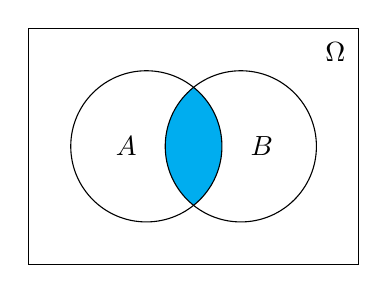
\begin{tikzpicture}[scale=.6]
\def\firstcircle{(180:1cm) circle (1.6cm)}
  \def\secondcircle{(0:1cm) circle (1.6cm)}
      \begin{scope}
      \clip\secondcircle; \fill[cyan] \firstcircle;
      \end{scope}
      \draw \firstcircle node[text=black,left] {$A$};
      \draw \secondcircle node [text=black,right] {$B$};
      \draw (-3.5,-2.5) rectangle (3.5,2.5);
      \node at (3,2) {$\Omega$};
\end{tikzpicture}
&

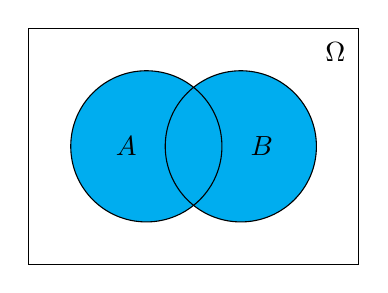
\begin{tikzpicture}[scale=.6]
\def\firstcircle{(180:1cm) circle (1.6cm)}
  \def\secondcircle{(0:1cm) circle (1.6cm)}
      \fill[cyan] \firstcircle;
      \fill[cyan] \secondcircle;
      \draw \firstcircle node[text=black,left] {$A$};
      \draw \secondcircle node [text=black,right] {$B$};
      \draw (-3.5,-2.5) rectangle (3.5,2.5);
      \node at (3,2) {$\Omega$};
\end{tikzpicture} \\
Venn diagram for $A \cap B$ & Venn diagram for $A \cup B$
\end{tabular}
\end{center}

\begin{center}
\begin{tabular}{l}
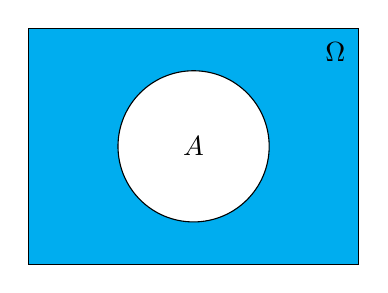
\begin{tikzpicture}[scale=.6]
\def\firstcircle{(0:0cm) circle (1.6cm)}
\def\mainrect{(-3.5,-2.5) rectangle (3.5,2.5)}
      \fill[cyan,even odd rule] \mainrect  \firstcircle;
      \draw \firstcircle node[text=black] {$A$};
          \draw \mainrect;
      \node at (3,2) {$\Omega$};
\end{tikzpicture} \\
Venn diagram for $A'$
\end{tabular}
\end{center}
\end{frame}

\begin{frame}{Example -- Three-Component System}
A system has three components, and to work either component A must work, \textit{or} both components B and C must work.

\begin{figure}
\centering
\parblk
{\blk{A}}
{\serblk{\blk{B}}{\blk{C}}}
\end{figure}

%$$\tikz[>=stealth] \graph [nodes={draw, rectangle}, layered layout,orient=2|3] {   
 % 1 -> {2,3}
%};$$
\pause We can use set theory to describe the event that the system works:
$$\text{System works} = A \cup (B \cap C)$$
where $A$, $B$, and $C$ represent the events that components A, B, and C work, respectively.

\vspace{.1in}
\pause We will come back to this problem again after introducing some probability theory.
\end{frame}


\begin{frame}{Venn Diagrams with Three Events}
To draw a Venn diagram involving three or more events, it may help to work step-by-step. For example, to draw a Venn diagram for $A\cup (B\cap C)$, first draw Venn diagrams for $A$ and $B \cap C$, then combine them to get the Venn diagram for $A \cup (B\cap C)$:

\vspace{.5cm}
\begin{tabular}{ccc}
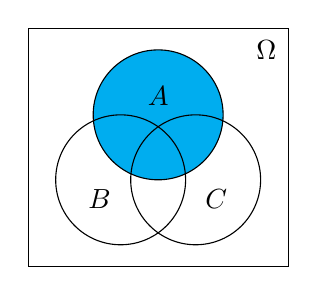
\begin{tikzpicture}[scale=.55]
\def\firstcircle{(90:1cm) circle (1.5cm)}
  \def\secondcircle{(210:1cm) circle (1.5cm)}
  \def\thirdcircle{(330:1cm) circle (1.5cm)}
      \fill[cyan] \firstcircle;
      \draw \firstcircle node[text=black,above] {$A$};
      \draw \secondcircle node [text=black,below left] {$B$};
      \draw \thirdcircle node [text=black,below right] {$C$};
      \draw (-3,-2.5) rectangle (3,3);
      \node at (2.5,2.5) {$\Omega$};
\end{tikzpicture}
&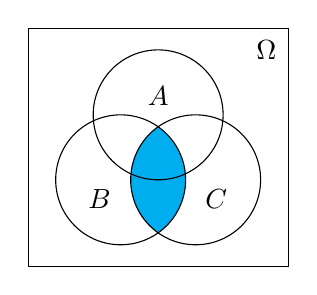
\begin{tikzpicture}[scale=.55]
\def\firstcircle{(90:1cm) circle (1.5cm)}
  \def\secondcircle{(210:1cm) circle (1.5cm)}
  \def\thirdcircle{(330:1cm) circle (1.5cm)}
    \begin{scope}
	\clip \secondcircle;
	\fill[cyan] \thirdcircle;
	\end{scope}
      \draw \firstcircle node[text=black,above] {$A$};
      \draw \secondcircle node [text=black,below left] {$B$};
      \draw \thirdcircle node [text=black,below right] {$C$};
      \draw (-3,-2.5) rectangle (3,3);
      \node at (2.5,2.5) {$\Omega$};
\end{tikzpicture}
&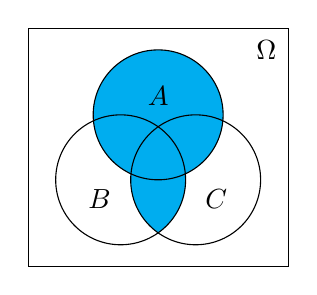
\begin{tikzpicture}[scale=.55]
\def\firstcircle{(90:1cm) circle (1.5cm)}
  \def\secondcircle{(210:1cm) circle (1.5cm)}
  \def\thirdcircle{(330:1cm) circle (1.5cm)}
    \fill[cyan] \firstcircle;
      \begin{scope}
    \clip \secondcircle;
    \fill[cyan] \thirdcircle;
      \end{scope}
      \draw \firstcircle node[text=black,above] {$A$};
      \draw \secondcircle node [text=black,below left] {$B$};
      \draw \thirdcircle node [text=black,below right] {$C$};
      \draw (-3,-2.5) rectangle (3,3);
      \node at (2.5,2.5) {$\Omega$};
\end{tikzpicture}\\
$A$ & $B \cap C$ & $A \cup (B \cap C)$
\end{tabular}
\end{frame}

%\begin{frame}{Example -- In Terms of Set Theory}
%
%In the example, $ \Omega=\{SSS, SSF, SFS, SFF, FSS, FSF, FFS, FFF\}  $, and we have events
%\begin{align*}
%A&=\{SFF,SFS,SSF,SSS\} &\text{Component A works}\\
%B&=\{FSF,FSS,SSF,SSS\}&\text{Component B works}\\
%C&=\{FFS,FSS,SFS,SSS\}&\text{Component C works}\\
%B\cap C &= \{FSS,SSS\}&\text{Components B,C work}\\
%A\cup(B\cap C) &= \{SFF,SFS,SSF,SSS,FSS\} &\text{System works}
%\end{align*}
%
%\begin{center}
%\begin{tabular}{m{2in}m{2in}}
%\begin{tikzpicture}
%\parblk
%{\blk{A}}
%{\serblk{\blk{B}}{\blk{C}}}
%\end{tikzpicture}
%&
%\begin{tikzpicture}[scale=.6]
%\def\firstcircle{(90:1cm) circle (1.5cm)}
%  \def\secondcircle{(210:1cm) circle (1.5cm)}
%  \def\thirdcircle{(330:1cm) circle (1.5cm)}
%      \fill[cyan] \firstcircle;
%      \begin{scope}
%    \clip \secondcircle;
%    \fill[cyan] \thirdcircle;
%      \end{scope}
%      \draw \firstcircle node[text=black,above] {$A$};
%      \draw \secondcircle node [text=black,below left] {$B$};
%      \draw \thirdcircle node [text=black,below right] {$C$};
%      \draw (-3,-2.5) rectangle (3,3);
%      \node at (2.5,2.5) {$\Omega$};
%\end{tikzpicture}
%\end{tabular}
%\end{center}
%
%\end{frame}

\begin{frame}{Disjoint events}
\begin{itemize}
\item The \emph{null event}, containing no outcomes, is denoted $\emptyset$.
\pause\item Two events $A$ and $B$ are \emph{disjoint} (or \emph{mutually exclusive}) if $A\cap B=\emptyset$, i.e., if they have no outcomes in common.
\pause\item For example, if we roll a die, let $A$ be the event that it is a 2 or lower and $B$ be the event that it is a 4 or higher:
\begin{align*}
A &= \{1,2\} \\
B &= \{4,5,6\}
\end{align*}
\end{itemize}

\begin{figure}
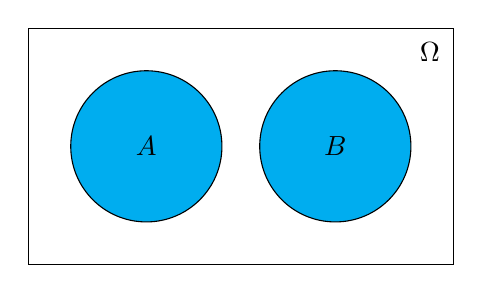
\begin{tikzpicture}[scale=.6]
\def\firstcircle{(180:2cm) circle (1.6cm)}
  \def\secondcircle{(0:2cm) circle (1.6cm)}
      \fill[cyan] \firstcircle;
      \fill[cyan] \secondcircle;
      \draw \firstcircle node[text=black] {$A$};
      \draw \secondcircle node [text=black] {$B$};
      \draw (-4.5,-2.5) rectangle (4.5,2.5);
      \node at (4,2) {$\Omega$};
\end{tikzpicture} \\
\caption{Venn diagram for $A \cup B$ when $A$ and $B$ are disjoint}
\end{figure}
\end{frame}

\begin{frame}{Several disjoint events}
Events $A_1,A_2,\dots,A_n$ are \emph{disjoint} if $A_i$ and $A_j$ are disjoint for every pair $i\neq j$.
\begin{figure}
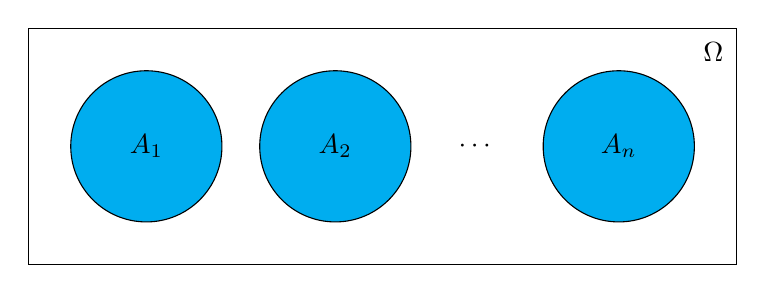
\begin{tikzpicture}[scale=.6]
\def\firstcircle{(0,0) circle (1.6cm)}
%  \def\secondcircle{(0:2cm) circle (1.6cm)}
  \def\secondcircle{(4cm,0) circle (1.6cm)}
  \def\thirdcircle{(10cm,0) circle (1.6cm)}
      \fill[cyan] \firstcircle;
      \fill[cyan] \secondcircle;
      \fill[cyan] \thirdcircle;
      \draw \firstcircle node[text=black] {$A_1$};
      \draw \secondcircle node [text=black] {$A_2$};
      \draw \thirdcircle node [text=black] {$A_n$};
      \draw (-2.5,-2.5) rectangle (12.5,2.5);
      \node at (12,2) {$\Omega$};
      \node at (7cm,0) {$\cdots$};
\end{tikzpicture} \\
\caption{Venn diagram for $A_1 \cup A_2 \cup \cdots \cup A_n$ when $A_1, A_2, \dots, A_n$ are disjoint}
\end{figure}
\end{frame}

\begin{frame}{Set-Theoretic Identities}
The following identities always hold for any events $A$, $B$, and $C$:

\begin{block}{}
\small \begin{tabular}{l|l}
$A \cap A = A$ & $A \cup A = A$ \\
$A \cap B = B \cap A$ &  $A \cup B = B \cup A$ \\ 
$A \cap (B \cap C) = (A \cap B) \cap C$ & $A \cup (B \cup C) = (A \cup B) \cup C$ \\
$A \cap (A \cup B) = A$ & $A \cup (A \cap B) = A$ \\
$A \cap (B \cup C) = (A \cap B) \cup (A \cap C)$ &
$A \cup (B \cap C) = (A \cup B) \cap (A \cup C)$ \\
$(A \cap B)' = A' \cup B'$ & $(A \cup B)' = A' \cap B'$  \\
$A \cap A' = \emptyset$ & $A \cup A' = \Omega$ \\
$A \cap \emptyset = \emptyset$ & $A \cup \Omega = \Omega$ \\
$A \cap \Omega = A$ & $A \cup \emptyset = A$ \\
$\emptyset' = \Omega$ & $\Omega' = \emptyset$ \\ 
$A'' = A$ & \\
\end{tabular}
\end{block}
\pause

You don't need to memorize these. We can use Venn diagrams to see why they are true:
\end{frame}


\begin{frame}{``Proof" that $A \cap (B \cup C) = (A \cap B) \cup (A \cap C)$}
\vspace{.1cm}
\hspace*{-.3cm}\begin{tabular}{ccc}
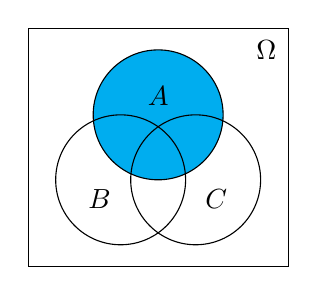
\begin{tikzpicture}[scale=.55]
\def\firstcircle{(90:1cm) circle (1.5cm)}
  \def\secondcircle{(210:1cm) circle (1.5cm)}
  \def\thirdcircle{(330:1cm) circle (1.5cm)}
      \fill[cyan] \firstcircle;
      \draw \firstcircle node[text=black,above] {$A$};
      \draw \secondcircle node [text=black,below left] {$B$};
      \draw \thirdcircle node [text=black,below right] {$C$};
      \draw (-3,-2.5) rectangle (3,3);
      \node at (2.5,2.5) {$\Omega$};
\end{tikzpicture}
&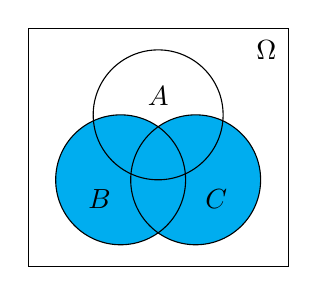
\begin{tikzpicture}[scale=.55]
\def\firstcircle{(90:1cm) circle (1.5cm)}
  \def\secondcircle{(210:1cm) circle (1.5cm)}
  \def\thirdcircle{(330:1cm) circle (1.5cm)}
	\fill[cyan] \secondcircle;
	\fill[cyan] \thirdcircle;
      \draw \firstcircle node[text=black,above] {$A$};
      \draw \secondcircle node [text=black,below left] {$B$};
      \draw \thirdcircle node [text=black,below right] {$C$};
      \draw (-3,-2.5) rectangle (3,3);
      \node at (2.5,2.5) {$\Omega$};
\end{tikzpicture}
&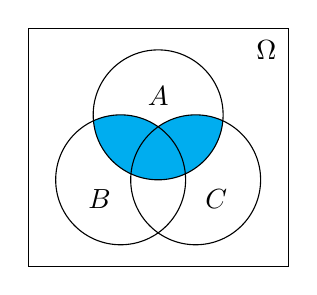
\begin{tikzpicture}[scale=.55]
\def\firstcircle{(90:1cm) circle (1.5cm)}
  \def\secondcircle{(210:1cm) circle (1.5cm)}
  \def\thirdcircle{(330:1cm) circle (1.5cm)}
      \begin{scope}
    \clip \firstcircle;
    \fill[cyan] \secondcircle;
    \fill[cyan] \thirdcircle;
      \end{scope}
      \draw \firstcircle node[text=black,above] {$A$};
      \draw \secondcircle node [text=black,below left] {$B$};
      \draw \thirdcircle node [text=black,below right] {$C$};
      \draw (-3,-2.5) rectangle (3,3);
      \node at (2.5,2.5) {$\Omega$};
\end{tikzpicture}\\
$A$ & $B \cup C$ & $A \cap (B \cup C)$\\
 \\
\vspace{.1cm}
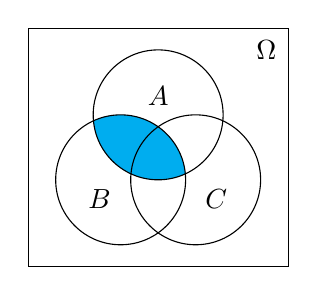
\begin{tikzpicture}[scale=.55]
\def\firstcircle{(90:1cm) circle (1.5cm)}
  \def\secondcircle{(210:1cm) circle (1.5cm)}
  \def\thirdcircle{(330:1cm) circle (1.5cm)}
      \begin{scope}
    \clip \firstcircle;
    \fill[cyan] \secondcircle;
      \end{scope}
      \draw \firstcircle node[text=black,above] {$A$};
      \draw \secondcircle node [text=black,below left] {$B$};
      \draw \thirdcircle node [text=black,below right] {$C$};
      \draw (-3,-2.5) rectangle (3,3);
      \node at (2.5,2.5) {$\Omega$};
\end{tikzpicture}
&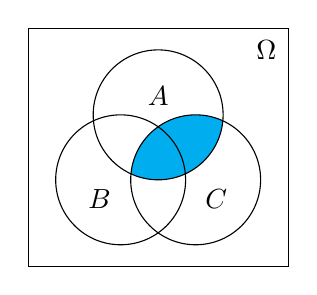
\begin{tikzpicture}[scale=.55]
\def\firstcircle{(90:1cm) circle (1.5cm)}
  \def\secondcircle{(210:1cm) circle (1.5cm)}
  \def\thirdcircle{(330:1cm) circle (1.5cm)}
      \begin{scope}
    \clip \firstcircle;
    \fill[cyan] \thirdcircle;
      \end{scope}
      \draw \firstcircle node[text=black,above] {$A$};
      \draw \secondcircle node [text=black,below left] {$B$};
      \draw \thirdcircle node [text=black,below right] {$C$};
      \draw (-3,-2.5) rectangle (3,3);
      \node at (2.5,2.5) {$\Omega$};
\end{tikzpicture}
&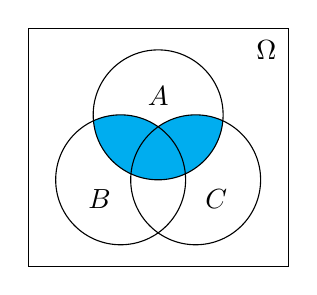
\begin{tikzpicture}[scale=.55]
\def\firstcircle{(90:1cm) circle (1.5cm)}
  \def\secondcircle{(210:1cm) circle (1.5cm)}
  \def\thirdcircle{(330:1cm) circle (1.5cm)}
      \begin{scope}
    \clip \firstcircle;
    \fill[cyan] \secondcircle;
    \fill[cyan] \thirdcircle;
      \end{scope}
      \draw \firstcircle node[text=black,above] {$A$};
      \draw \secondcircle node [text=black,below left] {$B$};
      \draw \thirdcircle node [text=black,below right] {$C$};
      \draw (-3,-2.5) rectangle (3,3);
      \node at (2.5,2.5) {$\Omega$};
\end{tikzpicture} \\
$A \cap B$ & $A \cap C$ & $(A \cap B) \cup (A \cap C)$
\end{tabular}\end{frame}

\begin{frame}{``Proof" that $(A \cap B)' = A' \cup B'$}
\begin{center}
\begin{tabular}{cc}
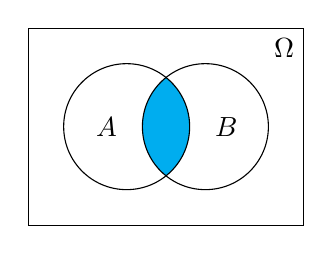
\begin{tikzpicture}[scale=.5]
\def\firstcircle{(180:1cm) circle (1.6cm)}
  \def\secondcircle{(0:1cm) circle (1.6cm)}
      \begin{scope}
      \clip \firstcircle;
      \fill[cyan] \secondcircle;
     \end{scope}
      \draw \firstcircle node[text=black,left] {$A$};
      \draw \secondcircle node [text=black,right] {$B$};
      \draw (-3.5,-2.5) rectangle (3.5,2.5);
      \node at (3,2) {$\Omega$};
\end{tikzpicture}
&
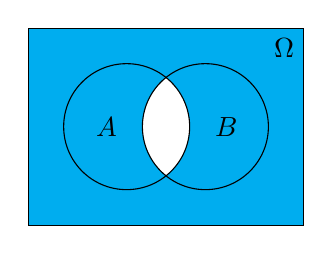
\begin{tikzpicture}[scale=.5]
\def\firstcircle{(180:1cm) circle (1.6cm)}
  \def\secondcircle{(0:1cm) circle (1.6cm)}
\def\mainrect{(-3.5,-2.5) rectangle (3.5,2.5)}
    \begin{scope}[even odd rule]
     \fill[cyan] \mainrect \firstcircle;
    \end{scope}
    \begin{scope}[even odd rule]
     \fill[cyan] \mainrect \secondcircle;
    \end{scope}
      \draw \firstcircle node[text=black,left] {$A$};
      \draw \secondcircle node [text=black,right] {$B$};
      \draw \mainrect;
      \node at (3,2) {$\Omega$};
\end{tikzpicture} \\
$A \cap B$ & $(A \cap B)'$
\end{tabular}
\end{center}

\begin{center}
\hspace*{-.5cm}\begin{tabular}{ccc}
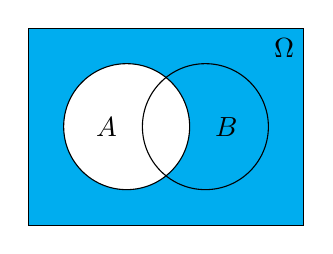
\begin{tikzpicture}[scale=.5]
\def\firstcircle{(180:1cm) circle (1.6cm)}
  \def\secondcircle{(0:1cm) circle (1.6cm)}
\def\mainrect{(-3.5,-2.5) rectangle (3.5,2.5)}
      \fill[cyan, even odd rule] \firstcircle \mainrect;
      \draw \firstcircle node[text=black,left] {$A$};
      \draw \secondcircle node [text=black,right] {$B$};
      \draw (-3.5,-2.5) rectangle (3.5,2.5);
      \node at (3,2) {$\Omega$};
\end{tikzpicture}
&
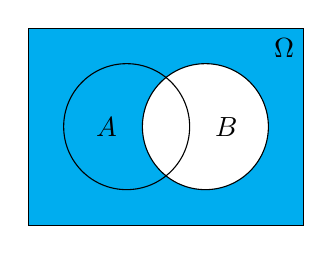
\begin{tikzpicture}[scale=.5]
\def\firstcircle{(180:1cm) circle (1.6cm)}
  \def\secondcircle{(0:1cm) circle (1.6cm)}
\def\mainrect{(-3.5,-2.5) rectangle (3.5,2.5)}
      \fill[cyan, even odd rule] \secondcircle \mainrect;
      \draw \firstcircle node[text=black,left] {$A$};
      \draw \secondcircle node [text=black,right] {$B$};
      \draw \mainrect;
      \node at (3,2) {$\Omega$};
\end{tikzpicture}
& 
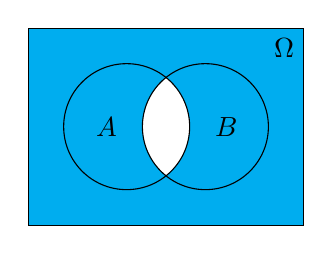
\begin{tikzpicture}[scale=.5]
\def\firstcircle{(180:1cm) circle (1.6cm)}
  \def\secondcircle{(0:1cm) circle (1.6cm)}
\def\mainrect{(-3.5,-2.5) rectangle (3.5,2.5)}
    \begin{scope}[even odd rule]
     \fill[cyan] \mainrect \firstcircle;
    \end{scope}
    \begin{scope}[even odd rule]
     \fill[cyan] \mainrect \secondcircle;
    \end{scope}
      \draw \firstcircle node[text=black,left] {$A$};
      \draw \secondcircle node [text=black,right] {$B$};
      \draw \mainrect;
      \node at (3,2) {$\Omega$};
\end{tikzpicture} \\
$A'$ & $B'$ & $A' \cup B'$
\end{tabular}
\end{center}
\end{frame}

\begin{frame}{``Proof" that $A\cap A'=\emptyset$ and $A\cup A'=\Omega$}
\begin{center}
\begin{tabular}{cc}
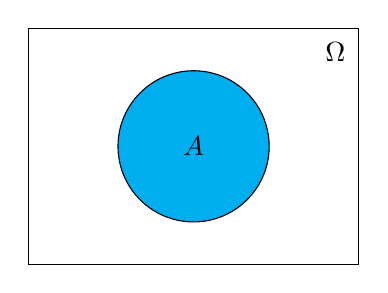
\begin{tikzpicture}[scale=.6]
\def\firstcircle{(0:0cm) circle (1.6cm)}
\def\mainrect{(-3.5,-2.5) rectangle (3.5,2.5)}
      \fill[cyan] \firstcircle;
      \draw \firstcircle node[text=black] {$A$};
          \draw \mainrect;
      \node at (3,2) {$\Omega$};
\end{tikzpicture} 
&
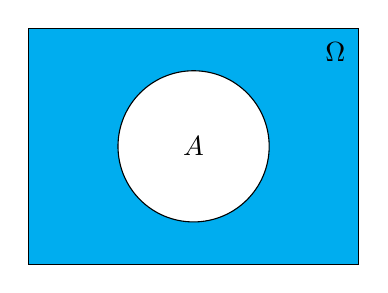
\begin{tikzpicture}[scale=.6]
\def\firstcircle{(0:0cm) circle (1.6cm)}
\def\mainrect{(-3.5,-2.5) rectangle (3.5,2.5)}
      \fill[cyan,even odd rule] \mainrect  \firstcircle;
      \draw \firstcircle node[text=black] {$A$};
          \draw \mainrect;
      \node at (3,2) {$\Omega$};
\end{tikzpicture} 
\\
$A$ & $A'$ \\
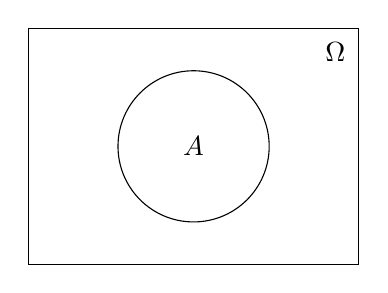
\begin{tikzpicture}[scale=.6]
\def\firstcircle{(0:0cm) circle (1.6cm)}
\def\mainrect{(-3.5,-2.5) rectangle (3.5,2.5)}
      \draw \firstcircle node[text=black] {$A$};
          \draw \mainrect;
      \node at (3,2) {$\Omega$};
\end{tikzpicture} 
&
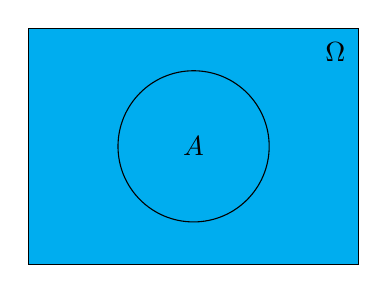
\begin{tikzpicture}[scale=.6]
\def\firstcircle{(0:0cm) circle (1.6cm)}
\def\mainrect{(-3.5,-2.5) rectangle (3.5,2.5)}
      \fill[cyan] \mainrect;
      \draw \firstcircle node[text=black] {$A$};
          \draw \mainrect;
      \node at (3,2) {$\Omega$};
\end{tikzpicture} 
\\
$A \cap A'=\emptyset$ & $A \cup A'=\Omega$
\end{tabular}
\end{center}
\end{frame}

\begin{frame}{``Proof" that $(A \cap B) \cap C = A \cap (B \cap C)$}

\vspace{.1cm}
\hspace*{-.3cm}\begin{tabular}{ccc}
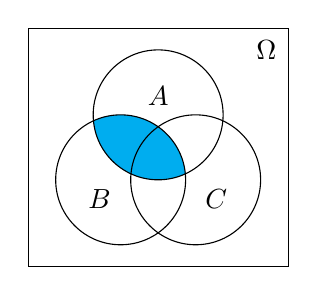
\begin{tikzpicture}[scale=.55]
\def\firstcircle{(90:1cm) circle (1.5cm)}
  \def\secondcircle{(210:1cm) circle (1.5cm)}
  \def\thirdcircle{(330:1cm) circle (1.5cm)}
      \begin{scope}
    \clip \secondcircle;
      \fill[cyan] \firstcircle;
      \end{scope}
      \draw \firstcircle node[text=black,above] {$A$};
      \draw \secondcircle node [text=black,below left] {$B$};
      \draw \thirdcircle node [text=black,below right] {$C$};
      \draw (-3,-2.5) rectangle (3,3);
      \node at (2.5,2.5) {$\Omega$};
\end{tikzpicture}
&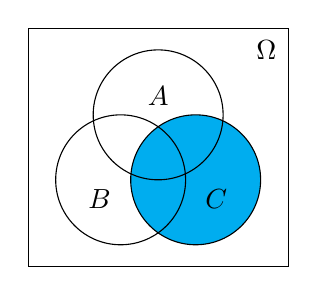
\begin{tikzpicture}[scale=.55]
\def\firstcircle{(90:1cm) circle (1.5cm)}
  \def\secondcircle{(210:1cm) circle (1.5cm)}
  \def\thirdcircle{(330:1cm) circle (1.5cm)}
      \fill[cyan] \thirdcircle;
      \draw \firstcircle node[text=black,above] {$A$};
      \draw \secondcircle node [text=black,below left] {$B$};
      \draw \thirdcircle node [text=black,below right] {$C$};
      \draw (-3,-2.5) rectangle (3,3);
      \node at (2.5,2.5) {$\Omega$};
\end{tikzpicture}
&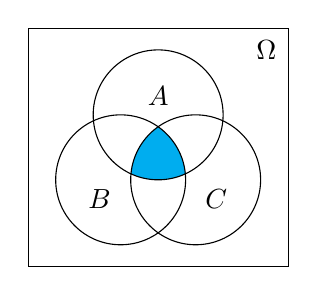
\begin{tikzpicture}[scale=.55]
\def\firstcircle{(90:1cm) circle (1.5cm)}
  \def\secondcircle{(210:1cm) circle (1.5cm)}
  \def\thirdcircle{(330:1cm) circle (1.5cm)}
      \begin{scope}
    \clip \firstcircle;
    \clip \secondcircle;
    \fill[cyan] \thirdcircle;
      \end{scope}
      \draw \firstcircle node[text=black,above] {$A$};
      \draw \secondcircle node [text=black,below left] {$B$};
      \draw \thirdcircle node [text=black,below right] {$C$};
      \draw (-3,-2.5) rectangle (3,3);
      \node at (2.5,2.5) {$\Omega$};
\end{tikzpicture}\\
$A \cap B$ & $C$ & $(A \cap B) \cap C$\\ \\
\vspace{.1cm}
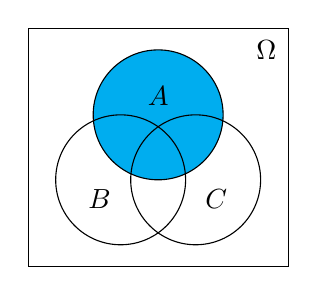
\begin{tikzpicture}[scale=.55]
\def\firstcircle{(90:1cm) circle (1.5cm)}
  \def\secondcircle{(210:1cm) circle (1.5cm)}
  \def\thirdcircle{(330:1cm) circle (1.5cm)}
      \fill[cyan] \firstcircle;
      \draw \firstcircle node[text=black,above] {$A$};
      \draw \secondcircle node [text=black,below left] {$B$};
      \draw \thirdcircle node [text=black,below right] {$C$};
      \draw (-3,-2.5) rectangle (3,3);
      \node at (2.5,2.5) {$\Omega$};
\end{tikzpicture}
&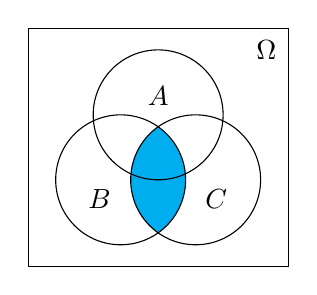
\begin{tikzpicture}[scale=.55]
\def\firstcircle{(90:1cm) circle (1.5cm)}
  \def\secondcircle{(210:1cm) circle (1.5cm)}
  \def\thirdcircle{(330:1cm) circle (1.5cm)}
      \begin{scope}
    \clip \secondcircle;
    \fill[cyan] \thirdcircle;
      \end{scope}
      \draw \firstcircle node[text=black,above] {$A$};
      \draw \secondcircle node [text=black,below left] {$B$};
      \draw \thirdcircle node [text=black,below right] {$C$};
      \draw (-3,-2.5) rectangle (3,3);
      \node at (2.5,2.5) {$\Omega$};
\end{tikzpicture}
&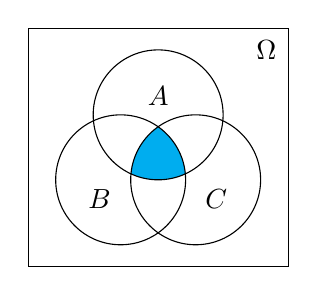
\begin{tikzpicture}[scale=.55]
\def\firstcircle{(90:1cm) circle (1.5cm)}
  \def\secondcircle{(210:1cm) circle (1.5cm)}
  \def\thirdcircle{(330:1cm) circle (1.5cm)}
      \begin{scope}
    \clip \firstcircle;
    \clip \secondcircle;
    \fill[cyan] \thirdcircle;
      \end{scope}
      \draw \firstcircle node[text=black,above] {$A$};
      \draw \secondcircle node [text=black,below left] {$B$};
      \draw \thirdcircle node [text=black,below right] {$C$};
      \draw (-3,-2.5) rectangle (3,3);
      \node at (2.5,2.5) {$\Omega$};
\end{tikzpicture} \\
$A$ & $B \cap C$ & $A \cap (B \cap C)$
\end{tabular}
\end{frame}

\begin{frame}{Multiple Intersections and Unions}
Since $(A \cap B) \cap C = A \cap (B \cap C)$, we don't need to use parentheses when writing the intersection of three or more events; we can simply write $A \cap B \cap C$. A similar statement applies to unions.

\begin{center}
\begin{tabular}{cc}
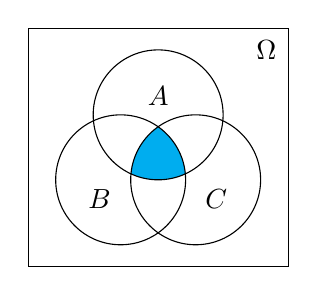
\begin{tikzpicture}[scale=.55]
\def\firstcircle{(90:1cm) circle (1.5cm)}
  \def\secondcircle{(210:1cm) circle (1.5cm)}
  \def\thirdcircle{(330:1cm) circle (1.5cm)}
      \begin{scope}
    \clip \firstcircle;
    \clip \secondcircle;
    \fill[cyan] \thirdcircle;
      \end{scope}
      \draw \firstcircle node[text=black,above] {$A$};
      \draw \secondcircle node [text=black,below left] {$B$};
      \draw \thirdcircle node [text=black,below right] {$C$};
      \draw (-3,-2.5) rectangle (3,3);
      \node at (2.5,2.5) {$\Omega$};
\end{tikzpicture}
&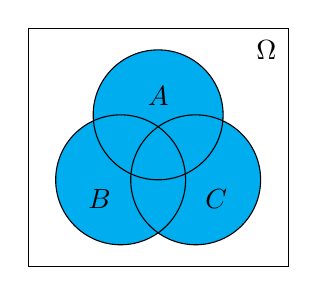
\begin{tikzpicture}[scale=.55]
\def\firstcircle{(90:1cm) circle (1.5cm)}
  \def\secondcircle{(210:1cm) circle (1.5cm)}
  \def\thirdcircle{(330:1cm) circle (1.5cm)}
    \fill[cyan] \firstcircle;
    \fill[cyan] \secondcircle;
    \fill[cyan] \thirdcircle;
      \draw \firstcircle node[text=black,above] {$A$};
      \draw \secondcircle node [text=black,below left] {$B$};
      \draw \thirdcircle node [text=black,below right] {$C$};
      \draw (-3,-2.5) rectangle (3,3);
      \node at (2.5,2.5) {$\Omega$};
\end{tikzpicture} \\
$A\cap B\cap C$ & $A \cup B \cup C$
\end{tabular}
\end{center}

\pause Caution: $A \cap (B \cup C)$ is \textit{not} the same as $(A \cap B) \cup C$. Parentheses must still be used to distinguish these.
\end{frame}

\begin{frame}{DeMorgan's Laws}
The following two identities are known as DeMorgan's laws:
\begin{align*}
(A \cap B)' &= A' \cup B' \\
(A \cup B)' &= A' \cap B'
\end{align*}
They also extend to three or more events:
\begin{align*}
(A \cap B \cap C)' &= A' \cup B' \cup C' \\
(A \cup B \cup C)' &= A' \cap B' \cap C'
\end{align*}
\end{frame}

\begin{frame}{Containment}
Given events $A$ and $B$, if every outcome in $A$ is also in $B$, then we say that $A$ is \emph{contained} in $B$, and we write $A \subseteq B$.

\begin{figure}
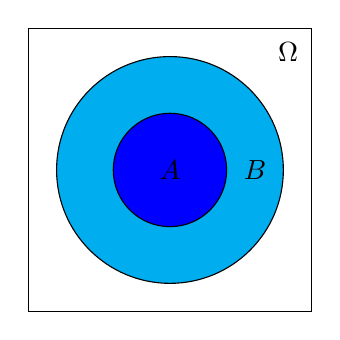
\begin{tikzpicture}[scale=.6]
\def\firstcircle{(0:0cm) circle (1.2cm)};
\def\secondcircle{(0:0cm) circle (2.4cm)}
\def\mainrect{(-3,-3) rectangle (3,3)}
      \fill[cyan] \secondcircle;
      \fill[blue] \firstcircle;
      \draw \firstcircle node[text=black] {$A$};
      \draw \secondcircle;
      \node at (1.8,0) {$B$};
          \draw \mainrect;
      \node at (2.5,2.5) {$\Omega$};
\end{tikzpicture} 
\end{figure}

\pause For example, if we roll a six-sided die, and let $A$ be the event of getting a 5 or higher and $B$ be the event of getting a 3 or higher, then $A \subseteq B$:
$$A=\{5,6\} \subseteq \{3,4,5,6\} = B$$
\end{frame}

\begin{frame}{Properties of Containment}
The following properties hold for any events $A$, $B$, and $C$: \begin{enumerate}
\item $A \subseteq A$.
\item $\emptyset \subseteq A$ and $A \subseteq \Omega$.
\item If $A \subseteq B$ and $B \subseteq C$, then $A \subseteq C$.
\item If $A\subseteq B$ and $B\subseteq A$, then $A=B$.
\item If $A\subseteq B$, then $A \cap B = A$ and $A \cup B = B$.
%\item $A \subseteq B$ if and only if $A\cap B =A$.
%\item $A \subseteq B$ if and only if $A\cup B =B$.
%\item $A \cup B \subseteq C$ if and only if $A\subseteq C$ and $B\subseteq C$.
%\item $A \subseteq B \cap C$ if and only if $A \subseteq B$ and $A \subseteq C$.
\item $A \subseteq A \cup B$ and $B \subseteq A\cup B$.
\item $A\cap B \subseteq A$ and $A \cap B \subseteq B$.
\item If $A\subseteq B$, then $A\cap C \subseteq B \cap C$ and $A \cup C \subseteq B \cup C$.
\item If $A\subseteq B$, then $B' \subseteq A'$.
\end{enumerate}
Again, you don't need to memorize these.
\end{frame}

\begin{frame}{Difference of Two Events}
Given events $A,B$ with $A\subseteq B$, we define their \emph{difference} $B - A$ as the set of all outcomes of $B$ which are not in $A$. In other words,
$$B-A = B \cap A'$$

This may be depicted using a Venn diagram:
\begin{center}
\begin{tabular}{c}
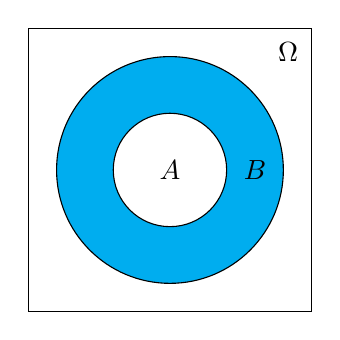
\begin{tikzpicture}[scale=.6]
\def\firstcircle{(0:0cm) circle (1.2cm)};
\def\secondcircle{(0:0cm) circle (2.4cm)}
\def\mainrect{(-3,-3) rectangle (3,3)}
      \fill[cyan] \secondcircle;
      \fill[white] \firstcircle;
      \draw \firstcircle node[text=black] {$A$};
      \draw \secondcircle;
      \node at (1.8,0) {$B$};
          \draw \mainrect;
      \node at (2.5,2.5) {$\Omega$};
\end{tikzpicture} \\
$B - A$
\end{tabular}
\end{center}
\end{frame}


%\begin{frame}{Set-Theoretic Algebra}
%We may use identities to simplify expressions involving events. For example,
%\begin{block}{}
%\vspace{-.5cm}\begin{align*}
%(A' \cap B)' \cap B 
%&= (A'' \cup B') \cap B \\
%&= (A \cup B') \cap B \\
%&= (A \cap B) \cup (B' \cap B) \\
%&= (A \cap B) \cup \emptyset \\
%&= A \cap B
%\end{align*}
%\end{block}
%
%\pause\begin{block}{}
%\vspace{-.5cm}\begin{align*}
%B' \cap (A \cup (A \cup B)')
%&= B' \cap (A \cup (A' \cap B')) \\
%&= B' \cap ((A \cup A') \cap (A \cup B')) \\
%&= B' \cap (\Omega \cap (A \cup B')) \\
%&= B' \cap (A \cup B') = B'
%\end{align*}
%\end{block}
%\end{frame}

%\begin{frame}{Quiz}
%Next class we'll have a quiz with three parts:
%\begin{enumerate}
%\item Set-theoretic identities: I'll give you the left-hand sides; you give me the right-hand sides.
%\item Venn diagrams: I'll ask you to use Venn diagrams to prove a certain identity (one in our list but not necessarily one proven in the slides).
%\item Set-theoretic algebra: I'll give you an expression, and you'll simplify it.
%\end{enumerate}
%See the Practice Quiz posted on Canvas.
%
%\begin{center}
%\includegraphics[scale=.2]{venn7.png}
%\end{center}
%\end{frame}

%\end{document} %%%%%%%%%%%%%%%%%%%%%%%%%%%%%%%%%%%%%

\begin{frame}{Interpretations of Probability}
What is ``probability"?
\pause\begin{tabular}{@{}p{8.5cm}p{1.5cm}}
\vspace{0cm}
Under the \emph{objective} interpretation, the probability of an event $A$ is the proportion of times that $A$ occurs when the experiment is repeated many times.
&
\vspace{0cm}
\includegraphics[scale=.1]{quarter.jpg}
\end{tabular}

\pause \begin{itemize}
\item For example, in tossing a coin, we say that the probability of getting heads is $.5$.
\item This only makes sense if the experiment can be repeated.
\end{itemize}
\pause 
\begin{tabular}{@{}p{8.5cm}p{1.5cm}}
\vspace{0cm}
Under the \emph{subjective} interpretation, probability is a 
measure of how likely a statement is to be true. 

\begin{itemize}
\item For example, someone says, ``There is a 70\% chance the Utes will beat Arizona this year."
\pause \item Different people may have different opinions and hence may assign different probabilities to the same statements.
\end{itemize}
&\vspace{0cm}
\includegraphics[scale=.3]{basketball.jpeg}
\end{tabular}
\end{frame}

\begin{frame}{Axioms of Probability}
The same mathematical theory applies to various interpretations of probability. Recall that given a set $\Omega$ of possible outcomes, subsets of $\Omega$ are called \emph{events}. We use the notation $P(A)$ to represent the probability of an event $A$, and we assume that probabilities satisfy the following axioms:
%\begin{block}{}
\begin{enumerate}
\item $P(A) \geq 0$
\item $P(\Omega)=1$
\item If $A_1, A_2,A_3,\dots$ are disjoint events, then
$$P(A_1\cup A_2\cup A_3\cup\dots) = \sum_{i=1}^\infty P(A_i)$$
\end{enumerate}
%\end{block}
\end{frame}

\begin{frame}{Equally Likely Outcomes}
Given a finite set $\Omega$ of outcomes, one of the simplest ways to define a probability measure is to assume that the outcomes are \emph{equally likely}:
$$P(A) = \frac{\# A}{\# \Omega} = \frac{\text{number of outcomes in $A$}}{\text{number of outcomes in $\Omega$}}$$

\pause \begin{example}
Suppose we roll a fair six-sided die. Let $\Omega=\{1,2,3,4,5,6\}$, and let $A=\{2,4,6\}$ be the event that we roll an even number. Then
$$P(A)=\frac{\# A}{\#\Omega}=\frac36=\frac12=.5$$
\end{example}
\pause Caution: It is not always reasonable to assume the outcomes are equally likely. %For example, in the three-component system example, we found $P(SFS)=.378$ but $P(FSF)=.012$.
\end{frame}

\begin{frame}{Example -- Sum of Two Dice}
\begin{problem}Suppose we roll two fair six-sided dice. What is the probability that they add up to 8?
\end{problem}

\pause\vspace{.5cm}There are 6 possibilities for the first roll and 6 possibilities for the second roll, so there are $6 \times 6 = 36$ equally likely outcomes:
$$\Omega=\{(1,1),(1,2),\dots,(1,6),(2,1),(2,2),\dots,(6,6)\}$$
\begin{tabular}{p{5cm}p{5cm}}
\begin{tabular}{l||p{.3cm}|p{.3cm}|p{.3cm}|p{.3cm}|p{.3cm}|p{.3cm}|}
& 1 & 2 & 3 & 4 & 5 & 6 \\ \hline \hline
1& 2 & 3 & 4 & 5 & 6 & 7 \\ \hline
2& 3 & 4 & 5 & 6 & 7 & \cellcolor{gray!15}8  \\ \hline
3& 4 & 5 & 6 & 7 & \cellcolor{gray!15}8 & 9 \\ \hline
4& 5 & 6 & 7 & \cellcolor{gray!15}8 & 9 & 10\\ \hline
5& 6 & 7 & \cellcolor{gray!15}8 & 9 & 10 & 11\\ \hline
6& 7 & \cellcolor{gray!15}8 & 9 & 10 & 11 & 12\\ \hline
\end{tabular}
& 
\begin{tabular}{p{5cm}}Out of these 36 possibilities, in 5 of them the dice add up 8. Therefore the probability that the dice add up to 8 is
$$P(A) = \frac{\# A}{\# \Omega} = \frac5{36} \approx .139$$
\end{tabular}
\end{tabular}
\end{frame}

\begin{frame}{Properties of Probability}
%As we'll show over the next few slides, t
The following properties of probability can be derived from the axioms:
\begin{enumerate}
\item $P(\emptyset)=0$, $P(\Omega)=1$.
\item If $A_1, \dots, A_n$ are disjoint events, then 
$$P(A_1 \cup \cdots \cup A_n)=P(A_1)+\cdots+P(A_n)$$ 
\item If $A \subseteq B$ then $P(B - A) = P(B)-P(A)$.
\item $A \subseteq B$ then $P(A) \leq P(B)$.
\item $0 \leq P(A) \leq 1$, for all events $A$.
\item $P(A') = 1-P(A)$ for any event $A$.
%\item $P(A\cup B)=P(A)+P(B)-P(A \cap B)$ for any events $A, B$.
\end{enumerate}
\end{frame}

%\begin{frame}{Properties of Probability}
%\begin{block}{}
%$P(\emptyset)=0$
%\end{block}
%\pause Recall the axioms:
%\begin{enumerate}
%\item $P(A) \geq 0$
%\item $P(\Omega)=1$
%\item $A_1, A_2,\dots$ disjoint $\implies$
%$P(A_1\cup A_2\cup\dots) = \sum_{i=1}^\infty P(A_i)$.
%\end{enumerate}
%\pause We know that
%$$\Omega = \Omega \cup \emptyset \cup \emptyset \cup \cdots$$
%\pause Therefore,
%\begin{align*}
%P(\Omega) &= P(\Omega)+P(\emptyset)+P(\emptyset)+\cdots \hfill & (\text{by axiom 3})\\
%&\geq P(\Omega)+P(\emptyset) \hfill & (\text{by axiom 1})
%\end{align*}
%\pause From $P(\Omega)\geq P(\Omega)+P(\emptyset)$ it follows that $0 \geq P(\emptyset)$. Since $P(\emptyset) \geq 0$ by axiom 1, it follows that $P(\emptyset)=0$.
%\end{frame}
%
%\begin{frame}{Properties of Probability}
%\begin{block}{}If $A_1, \dots, A_n$ are disjoint events, then 
%$$P(A_1 \cup \cdots \cup A_n)=P(A_1)+\cdots+P(A_n)$$ 
%\end{block}
%\pause We know that 
%$$A_1\cup\cdots\cup A_n = A_1\cup\cdots\cup A_n\cup\emptyset\cup\emptyset\cup\cdots$$
%and the events on the right side are disjoint.
%
%\pause Therefore,
%\begin{align*}
%P(A_1 \cup \cdots \cup A_n) &= P(A_1 \cup \cdots \cup A_n \cup\emptyset\cup\emptyset\cup\cdots)\\
%&= P(A_1)+\cdots+P(A_n)+P(\emptyset)+P(\emptyset)+\cdots \\
%&= P(A_1)+\cdots+P(A_n)+0+0+\cdots \\
%&= P(A_1)+\cdots+P(A_n)
%\end{align*}
%\end{frame}

%\begin{frame}{Properties of Probability}
%\begin{block}{}
%If $A\subseteq B$, then $P(B - A)=P(B)-P(A)$.
%\end{block}
%$A$ and $B-A$ are disjoint events with $B=A \cup (B-A)$. Therefore,
%\begin{align*}
%P(B)&=P(A \cup (B-A))\\
%&= P(A)+P(B-A)
%\end{align*}
%Rearranging this gives $P(B- A)=P(B)-P(A)$.
%\begin{center}
%\begin{tabular}{c}
%\begin{tikzpicture}[scale=.6]
%\def\firstcircle{(0:0cm) circle (1.2cm)};
%\def\secondcircle{(0:0cm) circle (2.4cm)}
%\def\mainrect{(-3,-3) rectangle (3,3)}
%      \fill[cyan] \secondcircle;
%      \fill[white] \firstcircle;
%      \draw \firstcircle node[text=black] {$A$};
%      \draw \secondcircle;
%      \node at (1.8,0) {$B$};
%          \draw \mainrect;
%      \node at (2.5,2.5) {$\Omega$};
%\end{tikzpicture} \\
%$B - A$
%\end{tabular}
%\end{center}
%\end{frame}

%\begin{frame}{Properties of Probability}
%\begin{block}{}
%\centering If $A \subseteq B$ then $P(A) \leq P(B)$.
%\end{block}
%\pause From the previous slide, $P(B-A)=P(B)-P(A)$, hence
%$$P(B)=P(A)+P(B-A) \geq P(A)$$
%
%\pause\begin{block}{}
%\centering $0 \leq P(A) \leq 1$, for all events $A$.
%\end{block}
%\pause Since $\emptyset \subseteq A \subseteq \Omega$, the previous property implies $$P(\emptyset) \leq P(A) \leq P(\Omega)$$
%Since $P(\emptyset)=0$ and $P(\Omega)=1$, this implies $0 \leq P(A) \leq 1$.
%
%\pause \begin{block}{}
%\begin{center}$P(A')=1-P(A)$\end{center}
%\end{block}
%\pause Given an event $A$, we always have $A\subseteq \Omega$, so we may apply the property from the last slide:
%$$P(A') = P(\Omega - A) = P(\Omega)-P(A)=1-P(A)$$
%\end{frame}

\begin{frame}{Probability of a Union of Two Events}
\begin{block}{}
$P(A\cup B)=P(A)+P(B)-P(A \cap B)$ for any events $A, B$.
\end{block}
Intuition: To find the probability of $A \cup B$, we add the probabilities of $A$ and $B$, but then we have double counted the intersection $A \cap B$, so we have to subtract that.

\vspace{.1cm}
\begin{center}
\begin{tabular}{c}
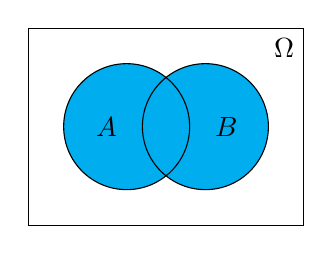
\begin{tikzpicture}[scale=.5]
\def\firstcircle{(180:1cm) circle (1.6cm)}
  \def\secondcircle{(0:1cm) circle (1.6cm)}
\def\mainrect{(-3.5,-2.5) rectangle (3.5,2.5)}
      \fill[cyan] \firstcircle \secondcircle;
      \draw \firstcircle node[text=black,left] {$A$};
      \draw \secondcircle node [text=black,right] {$B$};
      \draw (-3.5,-2.5) rectangle (3.5,2.5);
      \node at (3,2) {$\Omega$};
\end{tikzpicture} \\
 $A \cup B$
\end{tabular}
\end{center}
\end{frame}

\begin{frame}{Probability of a Union of Two Events}
\begin{block}{}
$P(A\cup B)=P(A)+P(B)-P(A \cap B)$ for any events $A, B$.
\end{block}

Proof: We may write $A\cup B$ as a union of two disjoint events: 
$$A\cup B = A \cup (B - (A \cap B))$$
Therefore, 
\begin{align*}
P(A\cup B) &= P(A \cup (B - (A \cap B))) \\
&= P(A) + P(B - (A \cap B)) \\
&= P(A) + P(B) - P(A\cap B) 
\end{align*}

\vspace{.1cm}
\hspace*{-.3cm}\begin{tabular}{ccc}
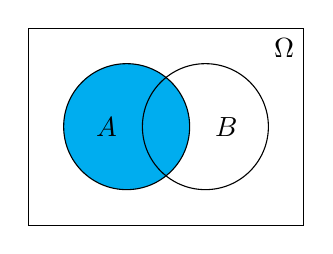
\begin{tikzpicture}[scale=.5]
\def\firstcircle{(180:1cm) circle (1.6cm)}
  \def\secondcircle{(0:1cm) circle (1.6cm)}
\def\mainrect{(-3.5,-2.5) rectangle (3.5,2.5)}
      \fill[cyan] \firstcircle ;
      \draw \firstcircle node[text=black,left] {$A$};
      \draw \secondcircle node [text=black,right] {$B$};
      \draw (-3.5,-2.5) rectangle (3.5,2.5);
      \node at (3,2) {$\Omega$};
\end{tikzpicture}
&
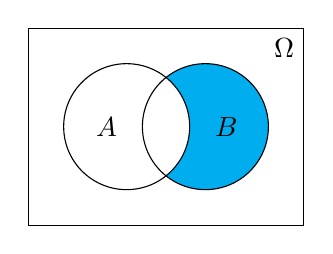
\begin{tikzpicture}[scale=.5]
\def\firstcircle{(180:1cm) circle (1.6cm)}
  \def\secondcircle{(0:1cm) circle (1.6cm)}
\def\mainrect{(-3.5,-2.5) rectangle (3.5,2.5)}
	\begin{scope}
	  \clip \secondcircle;
      \fill[cyan, even odd rule] \firstcircle \mainrect;
      \end{scope}
      \draw \firstcircle node[text=black,left] {$A$};
      \draw \secondcircle node [text=black,right] {$B$};
      \draw (-3.5,-2.5) rectangle (3.5,2.5);
      \node at (3,2) {$\Omega$};
\end{tikzpicture}&
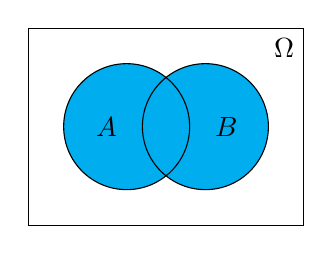
\begin{tikzpicture}[scale=.5]
\def\firstcircle{(180:1cm) circle (1.6cm)}
  \def\secondcircle{(0:1cm) circle (1.6cm)}
\def\mainrect{(-3.5,-2.5) rectangle (3.5,2.5)}
      \fill[cyan] \firstcircle \secondcircle;
      \draw \firstcircle node[text=black,left] {$A$};
      \draw \secondcircle node [text=black,right] {$B$};
      \draw (-3.5,-2.5) rectangle (3.5,2.5);
      \node at (3,2) {$\Omega$};
\end{tikzpicture} \\
$A$ & $B - (A\cap B)$ & $A \cup B$
\end{tabular}

\end{frame}

\begin{frame}{Probability of a Union of Three Events}
\begin{block}{}
\vspace{-.2in}\begin{align*}
P(A \cup B \cup C) = \ & P(A)+P(B)+P(C)\\
&-P(A \cap B)-P(A \cap C) - P(B \cap C) \\
&+ P(A\cap B\cap C)
\end{align*}
\end{block}

Intuition: To find the probability of $A \cup B \cup C$, we add the probabilities of the events $A$, $B$, and $C$ and subtract the overlap of each pair; but then we've subtracted the three-way overlap $A \cap B \cap C$ one too many times, so we add it back.

\vspace{.07in}
\begin{tabular}{p{1.3in}p{2.5in}}
%\begin{center}
\begin{tabular}[c]{c}
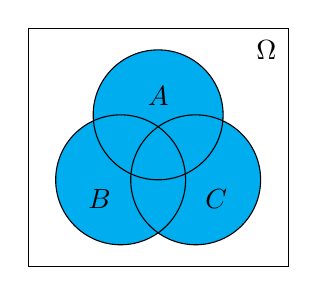
\begin{tikzpicture}[scale=.55]
\def\firstcircle{(90:1cm) circle (1.5cm)}
  \def\secondcircle{(210:1cm) circle (1.5cm)}
  \def\thirdcircle{(330:1cm) circle (1.5cm)}
    \fill[cyan] \firstcircle;
    \fill[cyan] \secondcircle;
    \fill[cyan] \thirdcircle;
      \draw \firstcircle node[text=black,above] {$A$};
      \draw \secondcircle node [text=black,below left] {$B$};
      \draw \thirdcircle node [text=black,below right] {$C$};
      \draw (-3,-2.5) rectangle (3,3);
      \node at (2.5,2.5) {$\Omega$};
\end{tikzpicture} \\
$A \cup B \cup C$
\end{tabular}
%\end{center}
& 
\begin{tabular}[c]{p{2.8in}}
P(A \cup B \cup C) = \ & P(A)+P(B)+P(C)\\
&-P(A \cap B)-P(A \cap C) - P(B \cap C) \\
&+ P(A\cap B\cap C)
\pause \textbf{Extra credit 1}: Prove this identity using only algebra, set-theoretic identities, and the formula $P(A \cup B)=P(A)+P(B)-P(A \cap B)$.

\vspace{.1in}
\pause \textbf{Extra credit 2}: Use this identity to solve problem 2.25 from the textbook.
\end{tabular}
\end{tabular}
\end{frame}


\begin{frame}{Examples}
Problems 2.12, 2.13, and 2.14.
\vspace{4in}
\end{frame}

%\end{document} % **********************************

\begin{frame}{Independence of Two Events}
\begin{definition}
Events $A$ and $B$ are \emph{independent} if
$P(A \cap B) = P(A)P(B)$.
\end{definition}
\pause\begin{example}
If we roll two fair six-sided dice and define events
\begin{align*}
A &= \text{first die is a six} \\
B &= \text{second die is a six}
\end{align*}
Then $A$ and $B$ are independent, $P(A)=1/6$, $P(B)=1/6$, so
$$P(\text{both dice are sixes}) = P(A\cap B)= P(A)P(B)=\frac16\cdot\frac16=\frac1{36}$$
\end{example}
\end{frame}

\begin{frame}{Dependence of Two Events}
\begin{example}
If we roll a fair six-sided dice and define events
\begin{align*}
A &= \text{the roll is a 4 or lower} \\
B &= \text{the roll is a 3 or higher}
\end{align*}
Then $P(A)=P(B)=\frac46=\frac23$ but $$P(A\cap B)=\frac26=\frac13 \neq \frac23\cdot\frac23=P(A)P(B)$$
So these two events are \textit{not} independent. We say that they are \emph{dependent}.
\end{example}

\textbf{Extra credit 3}: Based only on the outcome of a single roll of a fair six-sided die, find two events which are independent.
\end{frame}

\begin{frame}{Example}
\begin{problem}If we roll two fair six-sided dice, what is the probability that at least one of them is a six?
\end{problem}
Define events
\begin{align*}
A &= \text{first die is a 6}\\
B &= \text{second die is a 6}
\end{align*}
\pause Then
\begin{align*}
P(A\cup B)&=P(A)+P(B)-P(A\cap B) \\
&=P(A)+P(B)-P(A)P(B) \\
&=\frac16+\frac16-\left(\frac16\right)\left(\frac16\right) \\
&=\frac16+\frac16-\frac1{36} = \frac{11}{36} \approx .305
\end{align*}
\end{frame}

\begin{frame}{Independence of Several Events}
\begin{definition}
Events $A_1,\dots,A_n$ are \emph{independent} if
$$P(A_{i_1} \cap A_{i_2} \cap \cdots \cap A_{i_k}) = P(A_{i_1})P(A_{i_2})\cdots P(A_{i_k})$$
for all choices of indices $1\leq i_1 < i_2 < \cdots < i_k \leq n$
\end{definition}
\pause For example, saying three events $A, B, C$ are independent means 
\begin{align*}
P(A \cap B \cap C)&=P(A)P(B)P(C) \\
P(A \cap B)&=P(A)P(B) \\
P(A \cap C)&=P(A)P(C) \\
P(B \cap C)&=P(B)P(C)
\end{align*}
\end{frame}

\begin{frame}{Example -- Three-Component System}
\begin{center}
\begin{tabular}{p{1.5in}p{1.5in}}
\begin{tabular}{l}
\centering
\parblk
{\blk{A}}
{\serblk{\blk{B}}{\blk{C}}}
\end{tabular}
&
$\begin{aligned}
P(\text{A}) &= .7\\
P(\text{B}) &= .4\\
P(\text{C}) &= .9
\end{aligned}$
\end{tabular}
\end{center}

Assumed that failures in three components are independent of each other. Then, letting $A, B, C$ be the events that components A, B, and C work, respectively, we can solve the problem using the identity $P(X\cup Y)=P(X)+P(Y)-P(X \cap Y)$:
\pause \begin{align*}
P(\text{system works}) &= P(A\cup(B\cap C)) \\
&= P(A)+P(B\cap C)-P(A\cap B\cap C) \\
&= P(A)+P(B)P(C)-P(A)P(B)P(C) \\
&= .7+(.4)(.9)-(.7)(.4)(.9) = .808
\end{align*}
\end{frame}

%\begin{frame}{Example -- Three-Component System}
%Alternatively, we could note that 
%$$A\cup(B\cap C) = A\cup(A' \cap B \cap C)$$
%expresses the desired event as a union of two disjoint events, so we simply have
%\begin{align*}
%P(\text{system works}) &= P(A\cup(B\cap C)) \\
%&= P(A\cup(A'\cap B\cap C)) \\
%&= P(A) + P(A'\cap B\cap C) \\
%&= P(A) + P(A')P(B)P(C) \\
%&= .7 + (.3)(.4)(.9) = .808
%\end{align*}
%
%\pause Caution: If the system is vulnerable to potential failures which could affect multiple components (e.g., a power outage), then the assumption of independence may be inappropriate.
%\end{frame}

\begin{frame}{A Different Three-Component System}
\begin{center}
\begin{tabular}{p{1.5in}p{1.5in}}
\begin{tabular}{l}
\centering
\parblkt
{\blk{A}}
{\blk{B}}
{\blk{C}}
\end{tabular}
&
$\begin{aligned}
P(\text{A}) &= .7\\
P(\text{B}) &= .4\\
P(\text{C}) &= .9
\end{aligned}$
\end{tabular}
\end{center}

Now consider a new system where all three components are arranged in parallel, so that the system works as long as at least one of the three components does.

\pause\begin{align*}
P(\text{system works}) &= P(A\cup B\cup C) \\
%&= P((A\cup B\cup C)'') \\
&= 1- P((A\cup B\cup C)')\\
&= 1 - P(A' \cap B' \cap C')\\
&= 1-P(A')P(B')P(C') = 1-(.3)(.6)(.1) = .982
\end{align*}
This again assumes that the components work or fail independently of each other.
\end{frame}


%\begin{frame}{Independence Counterexample}
%Caution: Saying that several events are independent is \emph{not} equivalent to saying that each pair among them are independent.
%%\begin{example}
%
%\pause \vspace{.5cm} For example, suppose we roll two dice and define events
%\begin{align*}
%A &= \text{first die is a 6}\\
%B &= \text{second die is a 6}\\
%C &= \text{the two dice add up to 7}
%\end{align*}
%Then $P(A)=P(B)=P(C)=1/6$ and 
%\begin{align*}
%P(A\cap B)&=1/36=P(A)P(B)\\
%P(A\cap C)&=1/36=P(A)P(C)\\
%P(B\cap C)&=1/36=P(B)P(C)
%\end{align*}
%so each pair of the events 
%are independent. However,
%$$P(A \cap B \cap C)=0\neq 1/216 = P(A)P(B)P(C)$$
%%\end{example}
%\end{frame}
%
%\begin{frame}{Independence Counterexample}
%\textbf{Extra credit 4}: find an example of three events $A, B, C$ which are \textit{not} independent but such that
%$$P(A \cap B \cap C)=P(A)P(B)P(C)$$
%\end{frame}

\begin{frame}{Conditional Probability}
\begin{definition}
Let $B$ be an event with $P(B)>0$. The \emph{conditional probability} that an event $A$ occurs, given that $B$ occurs, is
$$P(A|B)=\frac{P(A\cap B)}{P(B)}$$
\end{definition}

For example, if we roll a fair six-sided die and let
\begin{align*}
A &= \text{we roll an even number} = \{2,4,6\}\\
B &= \text{we roll a 4 or higher} =\{4,5,6\}
\end{align*}
Then the conditional probability that we roll an even number, \textit{given} that we roll a 4 or higher, is
$$P(A|B) = \frac{P(A\cap B)}{P(B)} = \frac{1/3}{1/2} = \frac23 \approx .667$$
\end{frame}

\begin{frame}{Conditional Probability}
\begin{problem}
Suppose we roll two fair six-sided dice. What is the probability that one of the dice is a 6, given that the two dice sum to 8?
\end{problem}

\pause\begin{center}
\begin{tabular}{p{5cm}p{5.5cm}}
\begin{tabular}{l||p{.3cm}|p{.3cm}|p{.3cm}|p{.3cm}|p{.3cm}|p{.3cm}|}
& 1 & 2 & 3 & 4 & 5 & 6 \\ \hline \hline
1& 2 & 3 & 4 & 5 & 6 & 7 \\ \hline
2& 3 & 4 & 5 & 6 & 7 &  \cellcolor{cyan}8  \\ \hline
3& 4 & 5 & 6 & 7 &  \cellcolor{gray!15}8 & 9 \\ \hline
4& 5 & 6 & 7 &  \cellcolor{gray!15}8 & 9 & 10\\ \hline
5& 6 & 7 &  \cellcolor{gray!15}8 & 9 &10 & 11\\ \hline
6& 7 &  \cellcolor{cyan}8 & 9 & 10 & 11 & 12\\ \hline
\end{tabular}
&
$\begin{aligned}
&A = \text{one of the dice is a 6}\\
&B = \text{dice sum to 8}\\
&P(B) =  \frac5{36}\\
&P(A\cap B) = \frac2{36}\\
&P(A|B) = \frac{P(A\cap B)}{P(B)} = \frac{2/36}{5/36}=\frac25
\end{aligned}$
\end{tabular}
\end{center}
\end{frame}

\begin{frame}{Example -- Three-Component System}
\begin{center}
\begin{tabular}{p{1.5in}p{1.5in}}
\begin{tabular}{l}
\centering
\parblk
{\blk{A}}
{\serblk{\blk{B}}{\blk{C}}}
\end{tabular}
&
$\begin{aligned}
P(\text{A}) &= .7\\
P(\text{B}) &= .4\\
P(\text{C}) &= .9
\end{aligned}$
\end{tabular}
\end{center}

\begin{problem}
Suppose the above three-component system has failed. What is the probability that component B has failed?
\end{problem}

\vspace{-.5cm}
\pause
\begin{align*}
P(\text{system fails}) &= 1-P(\text{system works}) = 1-.808=.192 %\\[.3cm]
\end{align*}

\vspace{-.5cm}
\pause
\begin{align*}
P(B' \cap \text{system fails}) &= P(B' \cap (A \cup (B\cap C))') \\
&= P(B' \cap A' \cap (B' \cup C')) \\
&= P(B' \cap A') = P(B')P(A') = (.6)(.3) = .18 %\\[.3cm]
\end{align*}

\vspace{-.5cm}
\pause
\begin{align*}
P(B' | \text{system fails}) &= \frac{P(B' \cap \text{system fails})}{P(\text{system fails})}
= \frac{.18}{.192} = .9375
\end{align*}
\end{frame}

\begin{frame}{Independence and Conditional Probability}
Assume $A$ and $B$ are events with $P(B)>0$.
\begin{block}{}
$A$ and $B$ are independent if and only if $P(A|B)=P(A)$.
\end{block}
\pause In other words, saying $A$ and $B$ are independent means that knowing $B$ occurs doesn't change the probability that $A$ occurs.

\pause
\vspace{.5cm}Proof: By the definition of conditional probability,
\begin{align*}
P(A|B)=P(A) &\iff \frac{P(A\cap B)}{P(B)}=P(A) \\
&\iff P(A\cap B)=P(A)P(B) \\
&\iff \text{$A$ and $B$ are independent}
\end{align*}
\end{frame}

\begin{frame}{Multiplication Rule}
Assume $A$ is an event with $P(A)>0$.
\begin{block}{}
\vspace{-.2cm}$$P(A\cap B) = P(A)P(B|A)$$
\end{block}

\pause\vspace{.3cm}Proof: By the definition of conditional probability,
$$P(A)P(B|A) = P(A)\frac{P(A\cap B)}{P(A)}=P(A\cap B)$$
\end{frame}

\begin{frame}{Example}
\begin{tabular}{@{}p{8cm}p{3cm}}
\vspace{0cm}
A standard deck of 52 cards contains 4 aces. If you draw two cards at random, what is the probability that both will be aces?
&
\vspace{0cm}
\includegraphics[scale=.25]{cards.jpeg}
\end{tabular}

\vspace{.3cm}
\pause Define events
\begin{align*}
A &= \text{first card is an ace} \\
B &= \text{second card is an ace}
\end{align*}

Clearly $P(A)=4/52$. Then, given that the first card is an ace, there are only 3 aces among the 51 remaining cards, so $P(B|A)=3/51$. Therefore,
$$P(A\cap B)=P(A)P(B|A)=\frac4{52}\cdot\frac3{51}=\frac1{221}\approx .0045$$

\end{frame}

\begin{frame}{Multiplication Rule for Three Events}
The multiplication rule may be extended to three events:
\begin{block}{}
\vspace{-.2cm}$$P(A\cap B\cap C) = P(A)P(B|A)P(C|A\cap B)$$
\end{block}
\pause Proof: By the multiplication rule for two events,
\begin{align*}
P(A\cap B\cap C) &= P((A\cap B)\cap C) \\
&= P(A\cap B)P(C|A\cap B) \\ &= P(A)P(B|A)P(C|A\cap B)
\end{align*}

\pause\vspace{.2cm}
Example: Suppose we draw three cards at random. Let $A$, $B$, $C$ be the events that the first, second, and third cards are aces, respectively. Then
$$P(A)=4/52, P(B|A)=3/51, P(C|A\cap B)=2/50$$
Therefore, by the multiplication rule,
$$P(A\cap B\cap C) = \frac4{52}\cdot\frac3{51}\cdot\frac2{50}=\frac1{5525}$$
\end{frame}

\begin{frame}{Law of Total Probability}
\begin{block}{}
Let $A_1,\dots,A_n$ be disjoint events with $\Omega=A_1\cup\cdots\cup A_n$. Then for any event $B$,
$$P(B)=\sum_{i=1}^n P(A_i)P(B|A_i)$$
\end{block}

\pause Proof: By the multiplication rule, \begin{align*}
\sum_{i=1}^n P(A_i)P(B|A_i) &= 
\sum_{i=1}^n P(A_i \cap B) \\
&= P(A_1\cap B)+\cdots+P(A_n\cap B)\\
&= P((A_1\cap B)\cup\cdots\cup (A_n\cap B)) \\
&= P((A_1 \cup \cdots \cup A_n) \cap B) \\
&= P(\Omega \cap B) = P(B)
\end{align*}
\end{frame}

\begin{frame}{Example}
A manufacturer produces widgets using two machines in parallel: 70\% of widgets are produced by machine A; the rest are produced by machine B. Of the widgets produced by machine A, 3\% are defective; of those produced by machine B, 8\% are defective. If a random widget is chosen, what is the probability it is defective?

\pause\vspace{.3cm}
Solution: Define events
\begin{align*}
A &= \text{the widget is produced by machine A} \\
B &= \text{the widget is produced by machine B} \\
D &= \text{the widget is defective}
\end{align*}
Then the given information may be expressed,
$$P(A)=.7, P(B)=.3, P(D|A)=.03, P(D|B)=.08$$
\pause The law of total probability gives
$$P(D) = P(A)P(D|A)+P(B)P(D|B) = (.7)(.03)+(.3)(.08) = .045$$
\end{frame}

\begin{frame}{Bayes' Theorem}
How are $P(A|B)$ and $P(B|A)$ related?
\pause\begin{block}{}
\vspace{-.2cm}$$P(B|A) = \frac{P(A|B)P(B)}{P(A)} \quad\quad (\text{assuming $P(A)>0, P(B)>0$})$$
\end{block}
\pause Proof: By the multiplication rule,
$$P(B|A) = \frac{P(A \cap B)}{P(A)} = \frac{P(A|B)P(B)}{P(A)}$$

\pause Example: In the previous problem, if a randomly selected widget is defective, what is the probability it was produced by machine A?
\pause $$P(A|D) = \frac{P(D|A)P(A)}{P(D)} = \frac{(.03)(.7)}{.045}\approx .467$$
\end{frame}

\begin{frame}{Example -- Medical Testing}
A rare disease affects 1 in 1000 people. A person with the disease tests positive 99\% of the time, whereas a person without the disease tests positive only 2\% of the time.
\begin{problem}
If a randomly selected person tests positive, what is the probability that they have the disease?
\end{problem}
\pause The given information may be expressed,
%\begin{align*}
%&P(\text{disease}) = .001 \\
%&P(\text{test positive} \mid \text{disease}) = .99 \\
%&P(\text{test positive} \mid \text{no disease}) = .02
%\end{align*}
$$P(D) = .001, P(T|D)=.99, P(T|D')=.02$$
The law of total probability implies
\begin{align*}
P(T) &= P(T|D)P(D)+P(T|D')P(D') \\
&= (.99)(.001)+(.02)(.999) = .02097
\end{align*}
Bayes' theorem then implies
\begin{align*}
P(D|T) = \frac{P(T|D)P(D)}{P(T)}
= \frac{(.99)(.001)}{.02097} \approx .047
\end{align*}
\end{frame}

\begin{frame}{Summary}
\begin{itemize}
\item Set-theory notation: $A \cap B$, $A \cup B$, $A'$
\item Venn diagrams
%\item Properties of probability:
%\begin{itemize}
\item For any $A$ and $B$, $P(A\cup B)=P(A)+P(B)-P(A\cap B)$
\vspace{.1in}
\item If $A$ and $B$ are disjoint, $P(A \cup B)=P(A)+P(B)$.
\vspace{.1in}
\item If $A$ and $B$ are independent, $P(A\cap B)=P(A)P(B)$.
\vspace{.1in}
\item Conditional probability: $P(A|B) = \dfrac{P(A\cap B)}{P(B)}$
\vspace{.1in}
\item Multiplication rule: $P(A \cap B)=P(A)P(B|A)$
\vspace{.1in}
\item Bayes' Theorem: $P(B|A) = \dfrac{P(A|B)P(B)}{P(A)}$
\vspace{.1in}
\item Law of Total Probability: If $A_1,\dots,A_n$ are disjoint with $\Omega=A_1\cup\cdots\cup A_n$,
then $P(B)=\sum_{i=1}^n P(A_i)P(B|A_i)$.

%\end{itemize}
\end{itemize}
\end{frame}

% system of components

\end{document}
